% Niveau :      PCSI *
% Discipline :  Chimie Orga I
% Mots clés :   Spectrométrie UV-visible, Réactions acidobasiques

\begin{exercise}{Bleu de bromothymol}{2}{PCSI}
{Chimie générale,Réactions acidobasiques,Spectroscopie,UV-visible}{bermu}


Le bleu de bromothymol (BBT) est un indicateur de pH très utilisé en biologie pour mettre en évidence la présence de $\mathrm{CO_2}$. Vers $\text{pH} = 7.1$, il passe de sa forme acide jaune à sa forme basique bleue (notées $\mathrm{InH}$ et $\mathrm{In^{-}}$ respectivement) :\vspace{-.5em}
\begin{center}
        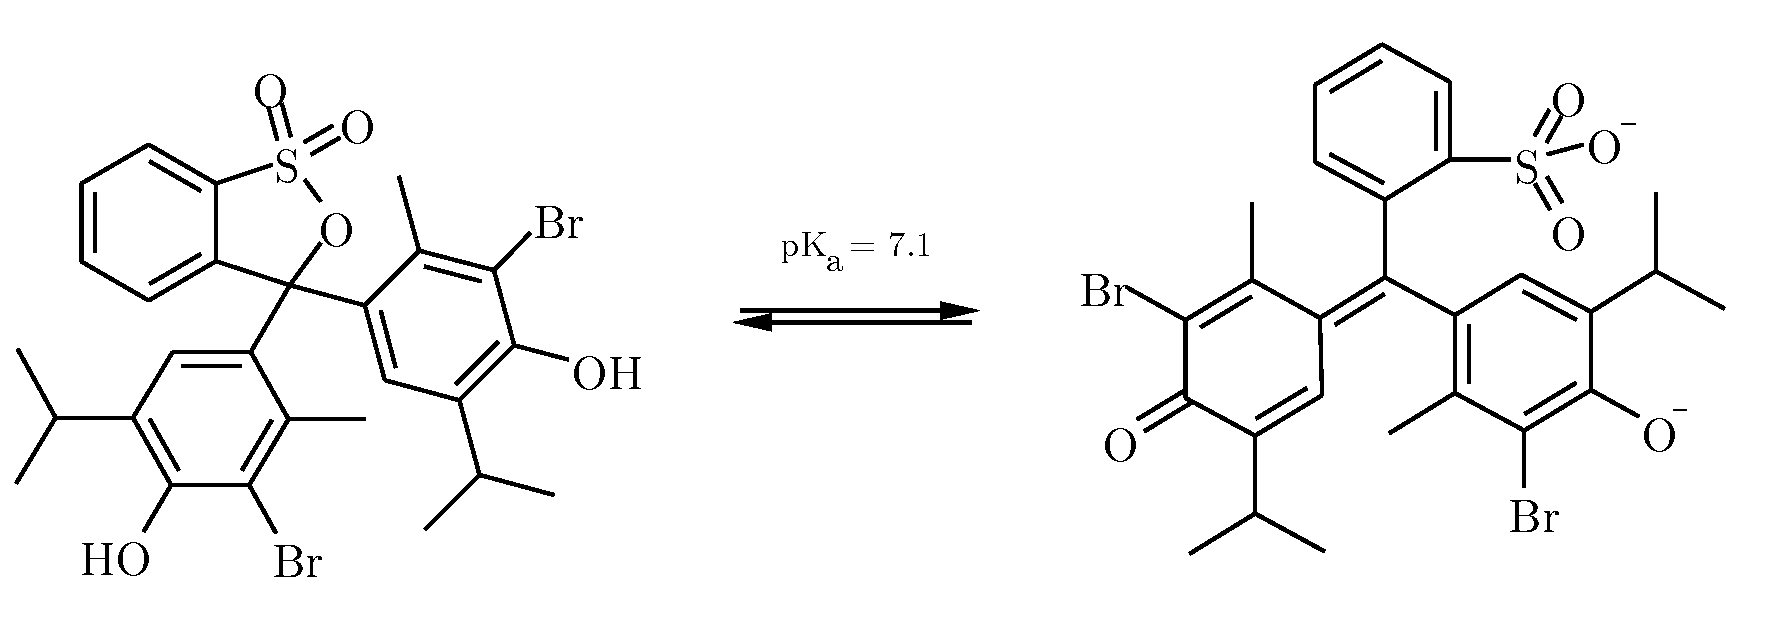
\includegraphics[width=.7\linewidth]{chimie/pH/BBT1.pdf}.\vspace{-1.5em}
\end{center}

\begin{questions}
\questioncours Théorie de Brönsted des acides et des bases. On précisera la définition du pK$_a$ et du pK$_e$.

\question Tracer le diagramme de prédominance de InH / In$^-$ en précisant la couleur de la solution dans chaque cas. Comparer à quelques exemples de couples acidobasiques connus.

\question Le CO$_2$ se comporte comme un diacide de pK$_a$ 6,4 et 10,3. \\ Tracer le diagramme de prédominance de CO$_2$ et discuter de l'utilisation du BBT pour la mise en évidence du CO$_2$ \textit{in vivo}.

\question\label{qu:1} Donner la relation entre le pH et le taux de dissociation $\alpha = \dfrac{\mathrm{[In^-]}}{\mathrm{[InH] + [In^-]}}$ du BBT.

\begin{EnvUplevel}
   On propose une méthodologie pour mesurer le pH d'une cellule par mesure de l'absorbance à l'aide du BBT :
    \begin{figure}[H]
        \centering
        \begin{tabularx}{\linewidth}{XX}
            \small{\textbf{(a)}} & \small{\textbf{(b)}}. \\
            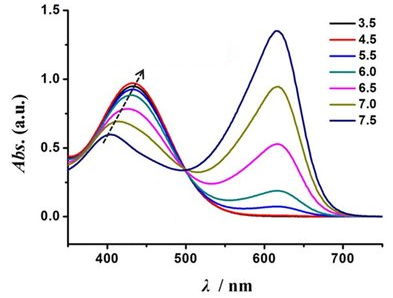
\includegraphics[width=\linewidth]{chimie/pH/BBT2.png} &
            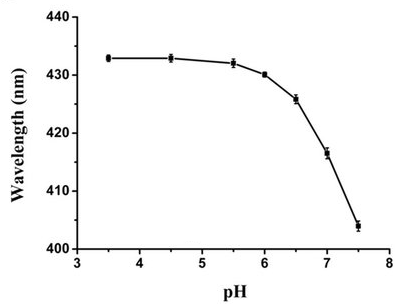
\includegraphics[width=\linewidth]{chimie/pH/BBT3.png}
        \end{tabularx}\vspace{-.5em}
        \caption{Spectres d'absorption UV-Visible (\textbf{a}) et courbe de calibration du pic à $\sim$ 420 nm (\textbf{b}) du bleu de bromothymol (BBT) pour différentes valeurs de pH. (Hui Hou, \emph{Nature Scientific Reports}, 7:1759, 2017)}
        \label{fig:BBT2}
    \end{figure}
\end{EnvUplevel}\vspace{-2ex}

\question Énoncer la loi de Beer--Lambert en précisant les hypothèses de validité.

\question Interpréter qualitativement la Fig.~(\textbf{a}) avec les deux maxima $\lambda_\text{max,a} = 433$ nm et {$\lambda_\text{max,b} = 616$~nm}.

\question\label{qu:2} Rappeler l'intérêt de mesurer l'absorbance au niveau des maxima d'intensité et justifier sans calcul que pour une seule espèce $i$
$$A_i(\lambda) \simeq A_{i,\text{max}}\,\qty(1 - \kappa_i\,\qty(\lambda - \lambda_{i,\text{max}})^2) \qqtext{pour} \lambda \simeq \lambda_{i,\text{max}},$$
$\kappa_i$ étant une constante qui dépend du chromophore à $\lambda_{i,\text{max}}$.

%\question Le point $\lambda_i = 500$ nm est nommé un point isobestique. Justifier par un simple calcul que ce point d'absorption constante $A_i$ durant la transformation $\mathrm{InH \xrightleftharpoons{} In^- + H^+}$ indique que cette transformation ne fait pas intervenir d'intermédiaire. \vspace{-2em}
%\begin{EnvUplevel}
%\paragraph{Indication :} exprimer l'absorbance de la solution en fonction des concentrations $[\mathrm{In^-}]$ et $[\mathrm{InH}]$.

%On va maintenant s'intéresser à modéliser la courbe de calibration.
%\end{EnvUplevel}

\question La forme basique du BBT possède également un maximum d'absorption en $\lambda_\text{max,b'} = 403$~nm. \\ A l'aide de la question \ref{qu:2}, donner l'absorption totale de la solution $A_\text{tot}$ en fonction de $\alpha$.

\question Donner longueur d'onde d'absorption maximale $\lambda_\text{max}$ en fonction de $\alpha$. Est-ce cohérent avec la Fig. (\textbf{b}) ?

%\question \`A l'aide de la relation d'Henderson--Hasselbalch et du $\mathrm{pK_a}$ du BBT, exprimer la relation $\lambda(\text{pH})$. \\

\end{questions}
\end{exercise}

\begin{solution}
\begin{questions}
    \questioncours
    \begin{itemize}
        \item Un acide de Brönsted est un donneur de H$^+$, une base de Brönsted est un accepteur de H$^+$ ;
        \item Le $K_a$ est la constante d'équilibre de la réaction
        \begin{center}\schemestart
        AH
        \arrow{<=>}[,1]
        A$^-$
        \+
        H$^+$
        \schemestop\chemnameinit{},\end{center}
        dont on déduit la relation de Henderson--Hasselbalch
        $$K_a = \mathrm{\dfrac{[A^-][H^+]}{[AH]}} \quad \Longleftrightarrow \quad \text{p}K_a = -\log K_a = \text{pH} + \log\mathrm{\dfrac{[A^-]}{[AH]}}.$$
        \item Le $K_e = 10^{-14}$ à 25$^\circ$C est la constante d'équilibre de la réaction d'autoprotolyse de l'eau
        \begin{center}\schemestart
        H$_2$O
        \arrow{<=>}[,1]
        H$^+$
        \+
        HO$^-$
        \schemestop\chemnameinit{},\end{center}
        dont on déduit la relation du produit ionique de l'eau
        $$K_e = \mathrm{[H^+][OH^-]}.$$
    \end{itemize}
    
    \question \hfill 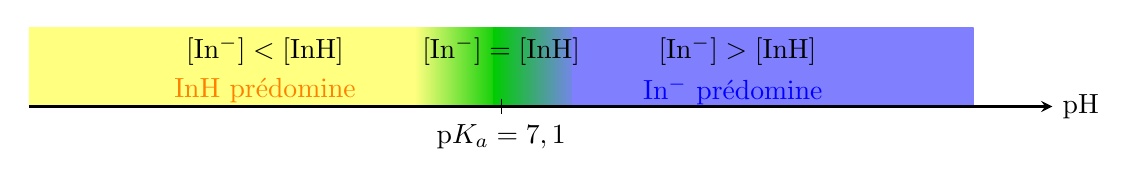
\begin{tikzpicture}[baseline=1em]
        \shade[left color = yellow!50, right color = yellow!50] (-6,0)rectangle(-1,1) ;
        \shade[left color = yellow!50, right color = green!80!black] (-1.1,0)rectangle(0,1) ;
        \shade[right color = blue!50, left color = green!80!black] (-.1,0)rectangle(1,1) ;
        \shade[right color = blue!50, left color =blue!50]
        (.9,0)rectangle(6,1) ;
        \node at (-3,.2) {\textcolor{orange}{InH prédomine}};
        \node at (3,.2) {\textcolor{blue}{$\mathrm{In^-}$ prédomine }};
        \draw[->, >=stealth, thick] (-6,0)--(7,0) node[right]{pH};
        \draw[black] (0,0.1)--(0,-0.1) node[below]{$\mathrm{p}K_a = 7,1$} ;
        \node at (-3,.7){$\left[ \mathrm{In^-}\right] < \left[ \mathrm{InH}\right]$};
        \node at (0,.7){$\left[ \mathrm{In^-}\right] = \left[ \mathrm{InH}\right]$};
        \node at (3,.7){$\left[ \mathrm{In^-}\right] > \left[ \mathrm{InH}\right]$};
    \end{tikzpicture} \hfill ~
    \newcommand{\tik}[4]{%
        \node[above] at (#1,.1){$\mathrm{#3}$};
        \node[above] at (#1,.9){$\mathrm{#4}$};
        \draw[black] (#1,0.1)--(#1,-0.1) node[below]{#2};
    }
    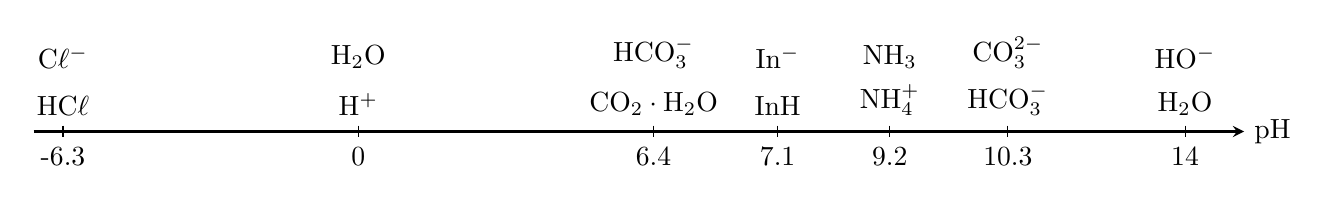
\begin{tikzpicture}[baseline=1em, scale=0.75]
        \draw[->, >=stealth, thick] (-5.5,0)--(15,0) node[right]{pH};
        \tik{-5}{-6.3}{HC\ell}{C\ell^-}
        \tik{0}{0}{H^+}{H_2O}
        \tik{14}{14}{H_2O}{HO^-}
        \tik{7.1}{7.1}{InH}{In^-}
        \tik{5}{6.4}{CO_2\cdot H_2O}{HCO_3^-}
        \tik{11}{10.3}{HCO_3^-}{CO_3^{2-}}
        \tik{9}{9.2}{NH_4^+}{NH_3}
    \end{tikzpicture}
    
    \question D'après la relation d'Henderson--Hasselbalch
    $$\text{p}K_a = \text{pH} + \log\mathrm{\dfrac{[In^-]}{[InH]}}
    = \text{pH} + \log\mathrm{\dfrac{[In^-]}{[In^-] + [InH]} \times \dfrac{[In^-] + [InH]}{[InH]}} = \text{pH} + \log\dfrac{\alpha}{1 - \alpha}.$$
    
    \question cf. \textbf{\sffamily Q2}. Le BBT devient jaune dès que le pH est inférieur à $\sim$ 7.1, or lorsqu'on dissout du CO$_2$, le pH baisse en dessous de 7, donc le BBT un indicateur adapté à cet usage.
    
    \question Pour des concentrations entre $10^{-3}$ M et $10^{-1}$ M, on a
    $$A(\lambda) = \ell\sum_i \varepsilon_i(\lambda) c_i,$$
    $A$ étant l'absorption de la solution, \\
    $\ell$ la taille de la cuve, \\
    $\varepsilon_i$ le coefficient d'absorption molaire du chromophore $i$, \\
    $c_i$ la concentration du composé $i$.
    
    \question La mesure au maximum d'absorption permet de minimiser l'erreur car $\Delta A \propto \Delta\lambda^2$ et de maximiser le signal par rapport au bruit.
    
    Pour $\lambda = \lambda_{i,\text{max}}$, $A_i = A_{i,\text{max}}$, et l'absorption diminue si on s'éloigne de $\lambda_{i,\text{max}}$ quadratiquement car on est à un max. 
    
    \question On remarque que la forme acide a un maximum d'absorption à $\lambda_\text{max,a} = 433$ nm dans le bleu (jaune en transmission), et la forme basique a un maximum d'absorption à $\lambda_\text{max,b} = 616$ nm dans le orange (bleu en transmission), ce qui est cohérent avec la couleur du BBT.
    
    \question $A_\text{tot} = \alpha A_{\text{max,b}}\,\qty(1 - \kappa_b\,\qty(\lambda - \lambda_{\text{max,b}})^2) + (1-\alpha) A_{\text{max,a}}\,\qty(1 - \kappa_a\,\qty(\lambda - \lambda_{\text{max,a}})^2)$
    
    \question $\displaystyle\eval{\pdv{A_\text{tot}}{\lambda}}_{\lambda_\text{max}} = 0 = 
    2\lambda_\text{max}\qty\bigg[\qty\Big(\gamma_a \lambda_\text{max,a} + \alpha (\gamma_b \lambda_\text{max,b} - \gamma_a \lambda_\text{max,a})) - \lambda_\text{max} \qty\Big(\gamma_a + \alpha(\gamma_b - \gamma_a))]$
    où  $\gamma_i = \kappa_i \varepsilon_i$
    $$\text{d'où}\qquad \lambda_\text{max} = \dfrac{\gamma_a \lambda_\text{max,a} + \alpha (\gamma_b \lambda_\text{max,b} - \gamma_a \lambda_\text{max,a})}{\gamma_a + \alpha(\gamma_b - \gamma_a)}
        = \lambda_\text{max,a} + \alpha \dfrac{\lambda_\text{max,b} - \lambda_\text{max,a}}{\gamma_a/\gamma_b + \alpha(1 - \gamma_a/\gamma_b)}$$
    ce qui est cohérent avec la figure b.
\end{questions}
\end{solution}